\documentclass[letterpaper, 12pt]{article}
\usepackage[margin=1in]{geometry}
\usepackage{graphicx}
\usepackage{listings}
\graphicspath{{images/}{../Template/images/}}
\lstset{language=[Motorola68k]assembler,basicstyle=\ttfamily,frame=single}

\newcommand{\hwnumber}{Lab 4}
\newcommand{\duedate}{October 20th, 2015}

\newcommand{\capper}{\begin{flushright}Aviles, Jean-Ralph \\ EEL3744 \\ Section 1539 \\ \duedate{} \\ \hwnumber{}\end{flushright}}

\begin{document}
\capper{}
\section*{Questions}
\begin{enumerate}
  \item What is the size of \textit{CS1} used in this lab? \\
    \hspace*{8pt} 64K - 0x470000:0x47FFFF
  \item What address lines \textbf{MUST} be present in the SRAM chip-enable equation for \textbf{full address decoding}? \\
    \hspace*{8pt} $A_{12}$ to $A_{23}$ are required as those are the ones that are constant for all 32K addresses in the SRAM.
  \item Draw a schematic of an \textbf{8}k x 8 RAM expansion starting at address 0x\textbf{9}000. \\ \underline{\textbf{You may only use address lines for decoding.}} \\
    \begin{center}
      \includegraphics[scale=0.1]{q3}
    \end{center}
  \item On the uPAD Proto Base board, is the CPLD required for interfacing with the SRAM? If not, explain. \\
    \hspace*{8pt} The CPLD is \textbf{not} required for interfacing with the SRAM. If we specify our Chip-select to exactly match the size of the device and we don't use any address decoding we can simply hook up the address and data lines, connect chip-enable to the chip select signal, and connect read and write enable to the signals from the XMEGA.
  \item The simple memory test program described above is not very good. It checks for neighboring data pins that are shorted or left unconnected, but we have no idea if the address bus is working. Describe a procedure for testing the address lines. Are there any limitations for your procedure (for example, does your procedure test \textbf{all} of the address lines)? Explain. \\
    \hspace*{8pt} One way we could test all the addresses is to write at every memory location first the lower bytes of the address used to index a location, check to ensure they are all correct, then move on to the next byte in the address and so on. This allows us to test to see that all addresses are correctly being accessed. If there are two addresses mapped to the same data location in the RAM then when you check the program on one of the passses you'll see that the byte you wrote to that location doesn't match up with what it was expected to be. this has no limitations and tests all the address lines used to index the RAM.
  \item In this lab, we configure \textbf{CS1} to be bigger than the SRAM so that we can divide it for multiple devices. If we want to connect many devices to the memory bus, this is a good way to conserve XMEGA chip select outputs. Suppose we wanted to configure \textbf{CS1} to span from 0x4\textbf{6}0000 to 0x47FFFF instead. Is this a valid range for an XMEGA chip select? With the hardware on your uPAD Proto Base as it is now, can we divide this new \textbf{CS1} the same way we do in this lab? Why or why not? \\
    \hspace*{8pt} First that range is valid $0x47FFFF - 0x460000 = 128K$ With the hardware on our Protobase as it is now we \textbf{cannot} divide this addres range since we only have access to $A_{15}:A_{0}$. To disambiguate all addresses in that range we would also need access to the $A_{16}$ address line.
\end{enumerate}
\section*{Problems Encountered}
Lots of sloppy errors with the Quartus design and a slight mistake in the configration for the chip selects caused me quite a bit of grief. But other than that everything went well.
\section*{Future Work/Applications}
Memory map all the things and add 16MB of external SRAM!
\section*{Appendix}
\subsection*{Part A}
\subsubsection*{Wiring diagram for Keypad}
\begin{center}
  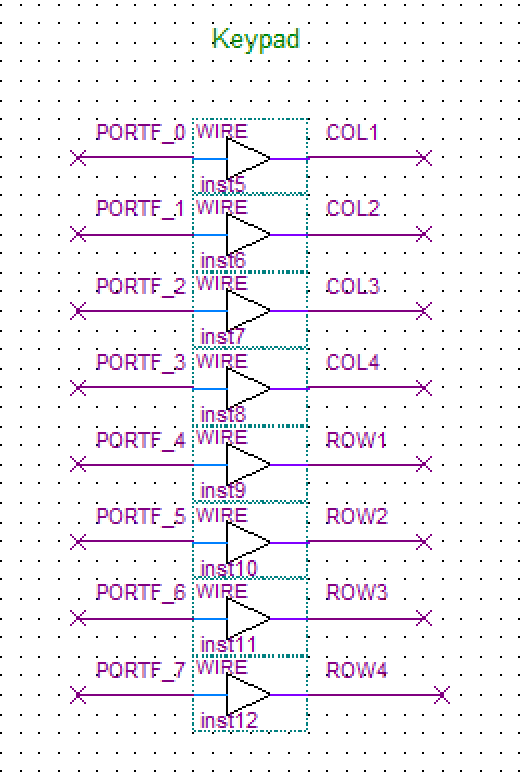
\includegraphics[scale=0.75]{keypad_schematic}
\end{center}
\subsection*{Part B}
\subsubsection*{Wiring diagram for SRAM}
\begin{center}
  \includegraphics[scale=0.1]{sram_wiring}
\end{center}
\pagebreak
\subsubsection*{Quartus Schematic}
\begin{center}
  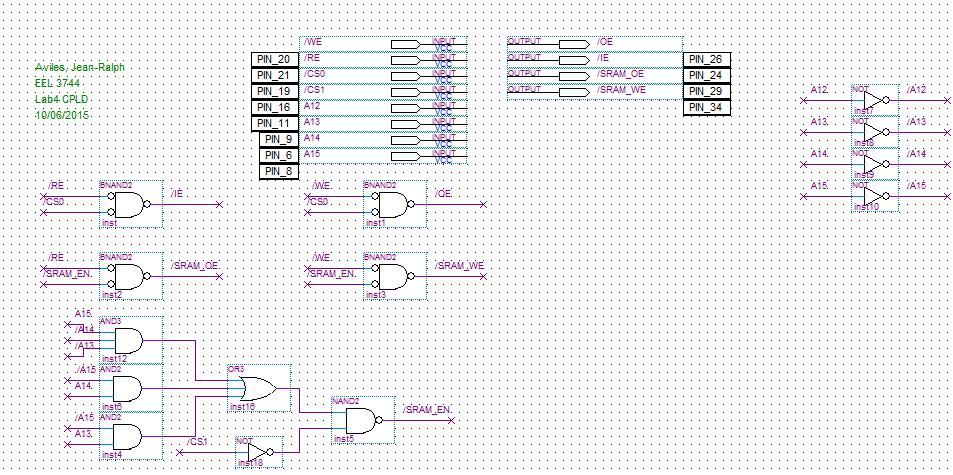
\includegraphics[scale=0.5]{lab4}
\end{center}
\section*{Pseudocode/Flowcharts}
\subsection*{Part A}
\subsubsection*{Pseudocode for reading from Keypad}
  \lstinputlisting{code/Lab4_keypad.ps}
\subsection*{Part B}
\subsubsection*{Pseudocode for part B}
  \lstinputlisting{code/Lab4_RAM.ps}
\section*{Programs}
\subsection*{Part A}
\subsubsection*{Assembly for reading from Keypad}
  \lstinputlisting{code/Lab4_keypad.asm}
\subsection*{Part B}
\subsubsection*{Assembly for part B}
  \lstinputlisting{code/Lab4_RAM.asm}
\end{document}
